\documentclass[a4paper,12pt,twoside]{memoir}

% Castellano
\usepackage[spanish,es-tabla]{babel}
\selectlanguage{spanish}
\usepackage[utf8]{inputenc}
\usepackage[T1]{fontenc}
\usepackage{lmodern} % Scalable font
\usepackage{microtype}
\usepackage{placeins}
\usepackage{listings}
\usepackage{subcaption}

\RequirePackage{booktabs}
\RequirePackage[table]{xcolor}
\RequirePackage{xtab}
\RequirePackage{multirow}

\usepackage[numbers,sort]{natbib}

% Links
\PassOptionsToPackage{hyphens}{url}\usepackage[colorlinks]{hyperref}
\hypersetup{
	allcolors = {red}
}

% Ecuaciones
\usepackage{amsmath}

% Rutas de fichero / paquete
\newcommand{\ruta}[1]{{\sffamily #1}}

% Párrafos
\nonzeroparskip

% Huérfanas y viudas
\widowpenalty100000
\clubpenalty100000

% Imágenes

% Comando para insertar una imagen en un lugar concreto.
% Los parámetros son:
% 1 --> Ruta absoluta/relativa de la figura
% 2 --> Texto a pie de figura
% 3 --> Tamaño en tanto por uno relativo al ancho de página
\usepackage{graphicx}
\newcommand{\imagen}[3]{
	\begin{figure}[!h]
		\centering
		\includegraphics[width=#3\textwidth]{#1}
		\caption{#2}\label{fig:#1}
	\end{figure}
	\FloatBarrier
}

% Comando para insertar una imagen sin posición.
% Los parámetros son:
% 1 --> Ruta absoluta/relativa de la figura
% 2 --> Texto a pie de figura
% 3 --> Tamaño en tanto por uno relativo al ancho de página
\newcommand{\imagenflotante}[3]{
	\begin{figure}
		\centering
		\includegraphics[width=#3\textwidth]{#1}
		\caption{#2}\label{fig:#1}
	\end{figure}
}

% El comando \figura nos permite insertar figuras comodamente, y utilizando
% siempre el mismo formato. Los parametros son:
% 1 --> Porcentaje del ancho de página que ocupará la figura (de 0 a 1)
% 2 --> Fichero de la imagen
% 3 --> Texto a pie de imagen
% 4 --> Etiqueta (label) para referencias
% 5 --> Opciones que queramos pasarle al \includegraphics
% 6 --> Opciones de posicionamiento a pasarle a \begin{figure}
\newcommand{\figuraConPosicion}[6]{%
  \setlength{\anchoFloat}{#1\textwidth}%
  \addtolength{\anchoFloat}{-4\fboxsep}%
  \setlength{\anchoFigura}{\anchoFloat}%
  \begin{figure}[#6]
    \begin{center}%
      \Ovalbox{%
        \begin{minipage}{\anchoFloat}%
          \begin{center}%
            \includegraphics[width=\anchoFigura,#5]{#2}%
            \caption{#3}%
            \label{#4}%
          \end{center}%
        \end{minipage}
      }%
    \end{center}%
  \end{figure}%
}

%
% Comando para incluir imágenes en formato apaisado (sin marco).
\newcommand{\figuraApaisadaSinMarco}[5]{%
  \begin{figure}%
    \begin{center}%
    \includegraphics[angle=90,height=#1\textheight,#5]{#2}%
    \caption{#3}%
    \label{#4}%
    \end{center}%
  \end{figure}%
}
% Para las tablas
\newcommand{\otoprule}{\midrule [\heavyrulewidth]}
%
% Nuevo comando para tablas pequeñas (menos de una página).
\newcommand{\tablaSmall}[5]{%
 \begin{table}
  \begin{center}
   \rowcolors {2}{gray!35}{}
   \begin{tabular}{#2}
    \toprule
    #4
    \otoprule
    #5
    \bottomrule
   \end{tabular}
   \caption{#1}
   \label{tabla:#3}
  \end{center}
 \end{table}
}

%
% Nuevo comando para tablas pequeñas (menos de una página).
\newcommand{\tablaSmallSinColores}[5]{%
 \begin{table}[H]
  \begin{center}
   \begin{tabular}{#2}
    \toprule
    #4
    \otoprule
    #5
    \bottomrule
   \end{tabular}
   \caption{#1}
   \label{tabla:#3}
  \end{center}
 \end{table}
}

\newcommand{\tablaApaisadaSmall}[5]{%
\begin{landscape}
  \begin{table}
   \begin{center}
    \rowcolors {2}{gray!35}{}
    \begin{tabular}{#2}
     \toprule
     #4
     \otoprule
     #5
     \bottomrule
    \end{tabular}
    \caption{#1}
    \label{tabla:#3}
   \end{center}
  \end{table}
\end{landscape}
}

%
% Nuevo comando para tablas grandes con cabecera y filas alternas coloreadas en gris.
\newcommand{\tabla}[6]{%
  \begin{center}
    \tablefirsthead{
      \toprule
      #5
      \otoprule
    }
    \tablehead{
      \multicolumn{#3}{l}{\small\sl continúa desde la página anterior}\\
      \toprule
      #5
      \otoprule
    }
    \tabletail{
      \hline
      \multicolumn{#3}{r}{\small\sl continúa en la página siguiente}\\
    }
    \tablelasttail{
      \hline
    }
    \bottomcaption{#1}
    \rowcolors {2}{gray!35}{}
    \begin{xtabular}{#2}
      #6
      \bottomrule
    \end{xtabular}
    \label{tabla:#4}
  \end{center}
}

%
% Nuevo comando para tablas grandes con cabecera.
\newcommand{\tablaSinColores}[6]{%
  \begin{center}
    \tablefirsthead{
      \toprule
      #5
      \otoprule
    }
    \tablehead{
      \multicolumn{#3}{l}{\small\sl continúa desde la página anterior}\\
      \toprule
      #5
      \otoprule
    }
    \tabletail{
      \hline
      \multicolumn{#3}{r}{\small\sl continúa en la página siguiente}\\
    }
    \tablelasttail{
      \hline
    }
    \bottomcaption{#1}
    \begin{xtabular}{#2}
      #6
      \bottomrule
    \end{xtabular}
    \label{tabla:#4}
  \end{center}
}

%
% Nuevo comando para tablas grandes sin cabecera.
\newcommand{\tablaSinCabecera}[5]{%
  \begin{center}
    \tablefirsthead{
      \toprule
    }
    \tablehead{
      \multicolumn{#3}{l}{\small\sl continúa desde la página anterior}\\
      \hline
    }
    \tabletail{
      \hline
      \multicolumn{#3}{r}{\small\sl continúa en la página siguiente}\\
    }
    \tablelasttail{
      \hline
    }
    \bottomcaption{#1}
  \begin{xtabular}{#2}
    #5
   \bottomrule
  \end{xtabular}
  \label{tabla:#4}
  \end{center}
}



\definecolor{cgoLight}{HTML}{EEEEEE}
\definecolor{cgoExtralight}{HTML}{FFFFFF}

%
% Nuevo comando para tablas grandes sin cabecera.
\newcommand{\tablaSinCabeceraConBandas}[5]{%
  \begin{center}
    \tablefirsthead{
      \toprule
    }
    \tablehead{
      \multicolumn{#3}{l}{\small\sl continúa desde la página anterior}\\
      \hline
    }
    \tabletail{
      \hline
      \multicolumn{#3}{r}{\small\sl continúa en la página siguiente}\\
    }
    \tablelasttail{
      \hline
    }
    \bottomcaption{#1}
    \rowcolors[]{1}{cgoExtralight}{cgoLight}

  \begin{xtabular}{#2}
    #5
   \bottomrule
  \end{xtabular}
  \label{tabla:#4}
  \end{center}
}



\graphicspath{ {./img/} }

% Capítulos
\chapterstyle{bianchi}
\newcommand{\capitulo}[2]{
	\setcounter{chapter}{#1}
	\setcounter{section}{0}
	\setcounter{figure}{0}
	\setcounter{table}{0}
	\chapter*{#2}
	\addcontentsline{toc}{chapter}{#2}
	\markboth{#2}{#2}
}

% Apéndices
\renewcommand{\appendixname}{Apéndice}
\renewcommand*\cftappendixname{\appendixname}

\newcommand{\apendice}[1]{
	%\renewcommand{\thechapter}{A}
	\chapter{#1}
}

\renewcommand*\cftappendixname{\appendixname\ }

% Formato de portada
\makeatletter
\usepackage{xcolor}
\newcommand{\tutor}[1]{\def\@tutor{#1}}
\newcommand{\course}[1]{\def\@course{#1}}
\definecolor{cpardoBox}{HTML}{E6E6FF}
\def\maketitle{
  \null
  \thispagestyle{empty}
  % Cabecera ----------------
\noindent
\includegraphics[width=\textwidth]{cabecera}\vspace{1cm}%
  \vfill
  % Título proyecto y escudo informática ----------------
  \colorbox{cpardoBox}{%
    \begin{minipage}{.8\textwidth}
      \vspace{.5cm}\Large
      \begin{center}
      \textbf{TFG del Grado en Ingeniería Informática}\vspace{.6cm}\\
      \textbf{\LARGE\@title{}}
      \end{center}
      \vspace{.2cm}
    \end{minipage}

  }%
  \hfill\begin{minipage}{.20\textwidth}
    
\includegraphics[width=\textwidth]{escudoInfor}
  \end{minipage}
  \vfill
  % Datos de alumno, curso y tutores ------------------
  \begin{center}%
  {%
    \noindent\LARGE
    Presentado por \@author{}\\ 
    en Universidad de Burgos --- \@date{}\\
    Tutor: \@tutor{}\\
  }%
  \end{center}%
  \null
  \cleardoublepage
  }
\makeatother

\newcommand{\nombre}{Miguel Fuente García} %%% cambio de comando

% Datos de portada
\title{Aplicación Android para la detección de retinopatía diabética}
\author{\nombre}
\tutor{D. Daniel Urda Muñoz y D. Nuño Basurto Hornillos}
\date{\today}

\begin{document}

\maketitle


\newpage\null\thispagestyle{empty}\newpage


%%%%%%%%%%%%%%%%%%%%%%%%%%%%%%%%%%%%%%%%%%%%%%%%%%%%%%%%%%%%%%%%%%%%%%%%%%%%%%%%%%%%%%%%
\thispagestyle{empty}


\noindent
\includegraphics[width=\textwidth]{cabecera}\vspace{1cm}

\noindent D. Daniel Urda Muñoz y D. Nuño Basurto Hornillos, profesores del departamento de Digitalización, área de Ciencia de la Computación e Inteligencia Artificial,

\noindent Exponen:

\noindent Que el alumno D. \nombre, con DNI 71313280D, ha realizado el Trabajo final de Grado en Ingeniería Informática titulado ``Aplicación Android para la detección de retinopatía diabética''. 

\noindent Y que dicho trabajo ha sido realizado por el alumno bajo la dirección del que suscribe, en virtud de lo cual se autoriza su presentación y defensa.

\begin{center} %\large
En Burgos, {\large \today}
\end{center}

\vfill\vfill\vfill

% Author and supervisor
\begin{minipage}{0.45\textwidth}
\begin{flushleft} %\large
Vº. Bº. del Tutor:\\[2cm]
D. Daniel Urda Muñoz
\end{flushleft}
\end{minipage}
\hfill
\begin{minipage}{0.45\textwidth}
\begin{flushleft} %\large
Vº. Bº. del co-tutor:\\[2cm]
D. Nuño Basurto Hornillos
\end{flushleft}
\end{minipage}
\hfill

\vfill

% para casos con solo un tutor comentar lo anterior
% y descomentar lo siguiente
%Vº. Bº. del Tutor:\\[2cm]
%D. nombre tutor


\newpage\null\thispagestyle{empty}\newpage




\frontmatter

% Abstract en castellano
\renewcommand*\abstractname{Resumen}
\begin{abstract}
La retinopatía diabética es una de las mayores causas de ceguera en los países desarrollados. Para diagnosticar el grado de la complicación, se realiza una imagen de la retina del paciente, captada por un retinógrafo. Esta prueba tiene un coste elevado para la sanidad pública, e implica a su vez que el paciente se desplace a un centro médico especializado. Así mismo, la cita con el especialista tiene una demora que puede perjudicar la situación del paciente. 

Por ello, se han desarrollado unos dispositivos, para las cámaras de los teléfonos móviles, que permiten obtener las fotografías de las retinas; de esta forma, el paciente no tendría que desplazarse a un hospital que disponga de un retinógrafo y el médico de familia podría realizar la fotografía al paciente, lo que facilitaría un posible cribado, anterior a la creación de la cita con el especialista. 

Este trabajo tiene como objetivo desarrollar una aplicación Android que facilite el trabajo del médico; permitiendo un primer diagnóstico del paciente mediante el envío de una imagen de la retina a modelos de aprendizaje computacional. De esta forma, los pacientes que tengan algún grado de retinopatía diabética, se les realice un estudio exhaustivo. 

Como resultado, se ha creado la aplicación RetinAI.


\end{abstract}

\renewcommand*\abstractname{Descriptores}
\begin{abstract}
Salud, retinopatía diabética, redes neuronales, aplicación Android.
\end{abstract}

\clearpage

% Abstract en inglés
\renewcommand*\abstractname{Abstract}
\begin{abstract}
Diabetic retinopathy is a leading cause of blindness in developed countries. To determine the degree of abnormality, the retinographer takes a image of patient's retina. This exam has a high cost for spanish public health, implying that the patient travels to a specialized medical center.

To address this, there are some lenses which have been developed for mobile phone cameras to take retina photos; this way, the patient would not have to go to a hospital that has a retinographand the family doctor could take the patient's photo, which would facilitate possible screening, prior to making an appointment with the specialist.

The objective of this work is to develop an Android app that help the doctor's work by allowing for an initial diagnosis of the patient through the submission of a retina image to computational learning models. This way, patients with any degree of diabetic retinopathy can undergo a comprehensive study.

As a result, the app RetinAI has been created.
\end{abstract}

\renewcommand*\abstractname{Keywords}
\begin{abstract}
Health, diabetic retinopathy, neural networks, Android app.
\end{abstract}

\clearpage

% Indices
\tableofcontents

\clearpage

\listoffigures

\clearpage

\listoftables
\clearpage

\mainmatter
\capitulo{1}{Introducción}

Durante los últimos años, se ha aumentado exponencialmente el uso de los dispositivos móviles, este aumento se debe principalmente a la comodidad que proporcionan respecto a otras tecnologías parecidas; siendo principalmente útiles para el uso de las redes sociales. 

Este aumento, tiene como consecuencia el fomento del desarrollo de aplicaciones móviles, puesto que, sin aplicaciones para estos dispositivos, no hubiesen tenido tanto auge. Estas aplicaciones están destinadas a dos sistemas operativos principalmente, que son Android e iOS; donde el 67,56\% de los usuarios prefieren Android y el 31.6\% iOS~\cite{mobile-os-market-share}.

Los móviles, no solo han sufrido un desarrollo significativo en lo referente a software, sino en hardware también, donde se han aumentado las características de procesador, cámara, RAM,... Y con ello, los desarrolladores
buscan crear aplicación que hagan uso de este hardware permitiendo muchas más funcionalidades. Una de estas funcionalidades es la integración de inteligencias artificiales que en los últimos años han reducido considerablemente los recursos y tiempo que necesitan para ejecutarse. Esta funcionalidad se ha convertido en una parte fundamental de la experiencia del usuario. Por ejemplo, aplicaciones de reconocimiento de voz como los asistentes virtuales (que utilizan algoritmos de procesamiento del lenguaje), también existen aplicaciones de reconocimiento facial para desbloquear el dispositivo (que se encuentra en el área de visión artificial) y el último ejemplo, son traducciones en tiempo real que facilitan la comunicación entre idiomas. Estos distintos usos que se dan a la inteligencia artificial están transformando la forma de interactuar con las aplicaciones móviles, brindando una experiencia más fluida y personalizada al usuario.

Por otro lado, la salud y bienestar han sido temas importantes para el ser humano; y por lo tanto, también se han hecho aplicaciones móviles con este objetivo. Como son aplicaciones del SACYL~\cite{sacyl-app}, de Adeslas~\cite{adeslas}, de la Organización Mundial de la salud~\cite{who-infoapp} y de Google~\cite{google-fitness-app} entre otras.


Además de las aplicaciones mencionadas anteriormente, también se han desarrollado otras más específicas destinadas a ayudar a las personas con discapacidad visual, la cual afecta a más de 2.200 millones de personas en el mundo. Las principales causas de pérdida de visión son la degeneración macular relacionada con la edad, las cataratas, la retinopatía diabética, el glaucoma y errores de refracción no corregidos. Unos 1.000 millones de personas tienen un deterioro moderado o grave de la visión\cite{oms-ceguera}.

La retinopatía diabética~\cite{enfermedad-ocular-diabetica} es una complicación de la diabetes, que afecta al sistema ocular del ser humano. Es causada por la inflamación, escape o cierre de los vasos sanguíneos de la retina, pudiendo desarrollarse nuevos vasos sanguíneos a lo largo del tiempo. Esta anomalía, encabeza las causas de ceguera en los países desarrollados. Según la Organización Mundial de la Salud, hasta 1 millón de personas tienen ceguera debido a la diabetes~\cite{oms-diabetes}. 
En Estados Unidos, cada año la retinopatía diabética suma un 12\% de nuevos casos de ceguera~\cite{porcentaje-afectados-eeuu}.
Hay varios grados de la patología de la retinopatía diabética entre los que se encontrarían por orden de menor a mayor peligrosidad~\cite{grados-retinopatia}: 
\begin{itemize}
    \item NPDR (Non-proloferative diabetic retinopathy), este grado se caracteriza por la ausencia de retinopatía;
    \item NPDR leve, donde los vasos sanguíneos empiezan a debilitarse, creando protuberancias llamadas micro-aneurismas;
    \item NPDR moderada, donde los vasos sanguíneos se siguen debilitando, se producen más hemorragias, pudiendo provocar visión borrosa;
    \item NPDR severa, en esta etapa, los vasos sanguíneos están dañados, causando falta de oxígeno en la retina y en la formación de nuevos vasos;
    \item PDR(proloferative diabetic retinopathy) o retinopatía diabética proliferativa, donde los vasos sanguíneos anormales que crecen en la retina y en el vítreo. Estos vasos pueden sangrar y provocar desprendimiento de retina, provocando la pérdida de visión.
\end{itemize} 

En el caso de la retinopatía diabética, también se han desarrollado aplicaciones móviles como Ret-iN CaM~\cite{ret-in-cam}, la cual permite guardar imágenes de las retinas de los pacientes, obteniendo un historial para realizar un estudio de la evolución de su patología. Esto es debido al desarrollo de una lente que permite obtener fotos de la retina desde el dispositivo móvil.


Actualmente cuando un paciente acude a su médico de familia por pérdida de visión, el médico le da cita para el especialista para que éste decida si se tiene que hacer una imagen del fondo de la retina con un retinógrafo, un dispositivo que permite obtener imágenes del fondo de la retina con una gran resolución, para descartar la posibilidad una retinopatía diabética. 
\markboth{Introducción}{Introducción}
Una vez que el paciente acude a la consulta del especialista (lo que puede llevar varios meses de espera con las consiguientes complicaciones), se podrán descartar muchas personas que no tienen la enfermedad. Pero todas estas pruebas y los recursos invertidos suponen elevados costes para la sanidad pública y demoras en el tiempo de espera de los pacientes que realmente tengan un grado de retinopatía diabética.
 
Por estos motivos, si el médico de familia utiliza la lente comentada anteriormente, junto con el teléfono móvil, se podrían obtener las imágenes del fondo de la retina, con la suficiente calidad como para hacer un diagnóstico preliminar. De esta manera se podrían reducir también los costes económicos comentados anteriormente y sobre todo el tiempo de espera de los pacientes al reducir las consultas que se derivan al especialista.


Como solución a este problema, siguiendo con la tendencia de aplicar los avances informáticos a la medicina, se propone realizar una aplicación móvil, que permita al médico de familia hacer un estudio, a partir de una foto de la retina del paciente, utilizando una lente para el dispositivo móvil~\cite{d-eyecare-lente}.
Además, para facilitar la labor del médico, esta aplicación móvil, proporciona redes neuronales convolucionales ya entrenadas, con las que el médico obtendrá un primer análisis del paciente, sabiendo cuándo la imagen tiene una calidad aceptable. De esta forma, se evitaría una lentitud en el sistema sanitario, enviando al especialista a aquellas personas que en cuyo resultado haya algún grado de retinopatía diabética. 
 

\section{Estructura}
La memoria se puede organizar en los siguientes apartados:
\begin{itemize}
    \item \textbf{Introducción}: Sección que dispone el tema y resume el contenido del trabajo.
    \item \textbf{Objetivos del proyecto}: Apartado donde se explican los objetivos que se buscan conseguir.
    \item \textbf{Conceptos teóricos}: Parte del documento donde se exponen los conceptos claves del proyecto.
    \item \textbf{Técnicas y herramientas}: Lugar donde se explican las metodologías y herramientas utilizadas durante la realización del proyecto.
    \item \textbf{Aspectos relevantes}: Capítulo donde se recogen los datos más importantes del desarrollo.
    \item \textbf{Trabajos relacionados}: Comparación del trabajo realizado, con otros anteriores.
    \item \textbf{Conclusiones y líneas de trabajo futuras}: Apartado donde se expone de forma critica el trabajo realizado, indicando posibles mejoras a realizar en un futuro.
\end{itemize}

Además, se adjunta como anexo los siguientes apartados:
\begin{itemize}
    \item \textbf{Plan de proyecto}: En este apartado donde se explica cómo se ha organizado el proyecto, y estudios sobre la rentabilidad tanto económica como legal tiene el proyecto.
    \item \textbf{Requisitos}: Parte del documento donde se explican los requisitos funcionales y no funcionales que tiene el proyecto.
    \item \textbf{Diseño}: Capítulo donde se describe la fase de diseño del proyecto.
    \item \textbf{Manual del programador}: Manual donde se recogen los aspectos que necesitaría un programador, tanto como para seguir el trabajo, como para poder entender el funcionamiento.
    \item \textbf{Manual del usuario}: Manual donde se realiza una guía de usuario, con los pasos a seguir para un correcto funcionamiento de la aplicación.
\end{itemize}

\capitulo{2}{Objetivos del proyecto}

Este apartado explica de forma precisa y concisa cuales son los objetivos que se persiguen con la realización del proyecto. Se puede distinguir entre los objetivos marcados por los requisitos del software a construir y los objetivos de carácter técnico que plantea a la hora de llevar a la práctica el proyecto.
\section{Objetivos generales}
\section{Objetivos técnicos}
\section{Objetivos personales}
\capitulo{3}{Conceptos teóricos}

En este proyecto, el enfoque principal se centra en las redes convolucionales, tanto en el preprocesado llevado, como la creación a través de transferencia de aprendizaje. Además, hay que tener en cuenta que se debe crear una aplicación Android, donde estas redes estén incluidas.

\section{Conceptos de Redes Neuronales}

    En esta sección, se van a ver los conceptos más importantes de las redes neuronales convolucionales en el contexto de la inteligencia artificial.

    La inteligencia artificial es una rama de la ciencia de la computación que trata de imitar la inteligencia humana para realizar tareas, buscando simular la capacidad de aprendizaje y razonamiento que tienen los seres humanos, entre otras cosas. Algunos de los objetivos de la inteligencia artificial son: representación de conocimientos, aprendizaje automático, procesamiento del lenguaje natural, inteligencia social e inteligencia general~\cite{definicion_artificial_intelligence}.

    El aprendizaje automático, o \textit{machine learning}, es una rama de la inteligencia artificial, cuyo objetivo es que las máquinas aprendan por sí mismas a partir de los datos proporcionados. Se considera aprendizaje a la adquisición de conocimientos a través del estudio, la  experiencia o de ser enseñado; como esta definición no es útil para las máquinas, se define nombrando rendimiento en vez de conocimiento, así, se considera que el objetivo del aprendizaje es mejorar el rendimiento en futuras acciones~\cite{machine-learning}.
    El aprendizaje automático se apoya en clasificadores para generar un modelo. Entre los más comunes se encuentran: los árboles de decisión, las reglas de asociación, los algoritmos genéticos, las máquinas de soporte vectorial, \textit{clustering}, las redes bayesianas y las redes neuronales artificiales.
    Según la naturaleza del aprendizaje automático, se puede considerar uno de estos tipos: aprendizaje supervisado, aprendizaje no supervisado, aprendizaje semisupervisado y aprendizaje por refuerzo.
    
    El aprendizaje supervisado es un tipo de aprendizaje automático, en este se dispone de un conjunto de datos junto con el resultado que se espera obtener. Durante el entrenamiento, el modelo aprende a reconocer patrones y relaciones entre los datos de entrada y sus respectivas etiquetas, si el modelo está proporcionando resultados incorrectos, se pueden corregir de forma que se obtengan mejores resultados. Con el modelo ya entrenado, se pueden obtener predicciones de datos no vistos. Un problema que surge es el \textit{overfitting}, el cual hace que el modelo aprenda los datos, dando los resultados correspondientes para cada instancia.

    El aprendizaje supervisado se ha beneficiado enormemente de los avances en las redes neuronales artificiales (RNN). Estas redes son modelos computacionales  con al menos una capa oculta~\cite{definicion_neural_network}, la cual consiste en una o más neuronas donde cada una calcula la suma de los valores de entrada, multiplicados por su peso correspondiente~\cite{definicion_hidden_layer}. En la figura~\ref{fig:funcionamientoRedNeuronal}, se puede observar una red neuronal, donde cada círculo representa una neurona artificial, y las flechas la conexión entre las distintas neuronas.

    \begin{figure}[!ht]
         \centering
         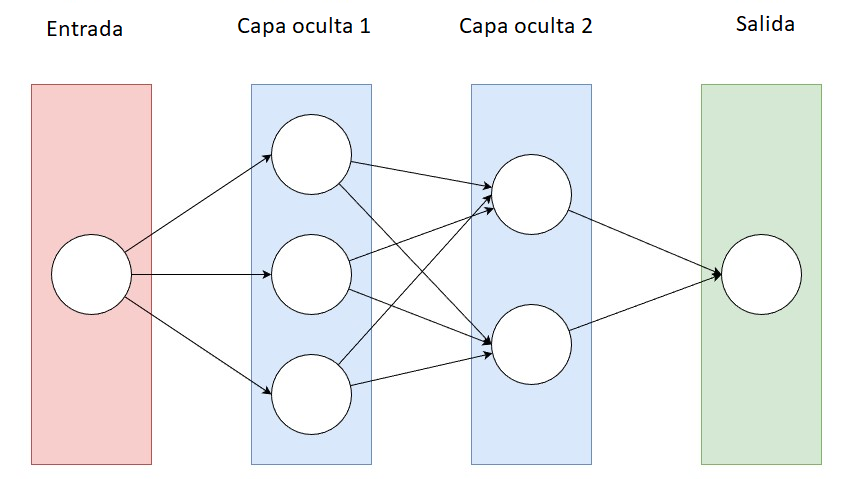
\includegraphics[width=0.9\textwidth]{img/RedNeuronal.png}
         \caption{Funcionamiento de una red neuronal}
         \label{fig:funcionamientoRedNeuronal}
    \end{figure}
    El valor calculado se utiliza en una función de activación, que produce el valor de salida\cite{definicion_activation_function}. Entre las funciones de activación destacan las visibles en \ref{fig:funciones_de_activacion}.
    \begin{itemize}
        \item La función RELU (verde), la cual indica el máximo entre 0 y el valor calculado~\ref{fig:funcionRELU}.
        \item La función lineal(rosa), la cual devuelve el mismo valor calculado~\ref{fig:funcionLineal}.
        \item La función sigmoidea(cían), la cual devuelve un valor entre 0 y 1 según lo alejado que este del 0~\ref{fig:funcionSigmoidal}.
        \item La función escalón(morada), devuelve o 0 o 1 dependiendo del signo del valor calculado~\ref{fig:funcionEscalon}.
    \end{itemize}
    
 \begin{figure}[!ht]
        \centering
        \begin{subfigure}{0.45\textwidth}
            \centering
            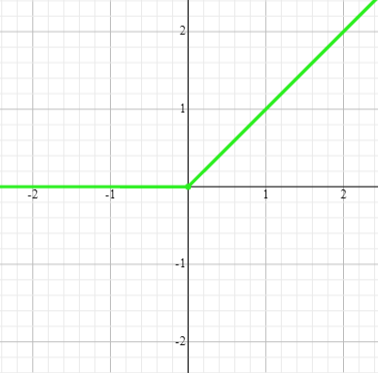
\includegraphics[width=\textwidth]{img/RELU.png}
            \caption{RELU}
            \label{fig:funcionRELU}
        \end{subfigure}
        \begin{subfigure}{0.45\textwidth}
            \centering
            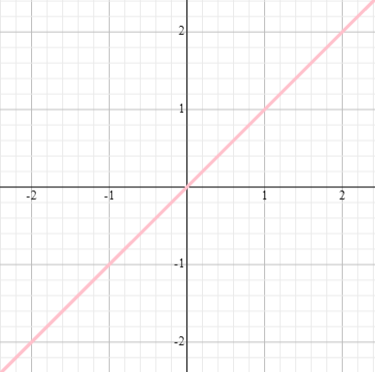
\includegraphics[width=\textwidth]{img/lineal.png}
            \caption{Lineal}
            \label{fig:funcionLineal}
        \end{subfigure}

        \vspace{1em}

        \begin{subfigure}{0.45\textwidth}
            \centering
            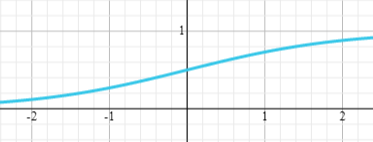
\includegraphics[width=\textwidth]{img/Sigmoidal.png}
            \caption{Sigmoidea}
            \label{fig:funcionSigmoidal}
        \end{subfigure}
        \begin{subfigure}{0.45\textwidth}
            \centering
            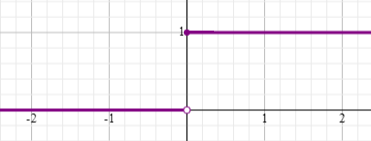
\includegraphics[width=\textwidth]{img/escalon.png}
            \caption{Escalón}
            \label{fig:funcionEscalon}
        \end{subfigure}

        \caption{Funciones de activación}
        \label{fig:funciones_de_activacion}
    \end{figure}

    Para hacer más visual una red neuronal, se hará un ejemplo, suponemos una asignatura, donde un alumno realiza 2 exámenes, 2 trabajos prácticos y 1 trabajo final. La nota final de la asignatura se corresponde a un 50\% de los exámenes, donde el primer examen vale un 40\% y el segundo un 60\%, un 30\% a los trabajos prácticos, donde ambos tienen el mismo porcentaje, y el trabajo final que vale un 20\%. 
    
    El profesor de la asignatura quiere saber si un alumno ha aprobado o suspendido, con las siguientes notas: un 8 en el primer examen, un 1 en el segundo, en ambos trabajos prácticos un 5 y en el trabajo final un 6.

    En la figura  \ref{fig:ejemploRedNeuronal} se observa la ejemplificación de la red, donde la capa roja se corresponde a la capa de entrada, la capa azul con la capa oculta de la red, y la capa verde con la capa de salida. En este caso, en la capa oculta se ha usado una función de activación RELU, obteniendo los valores de dentro de los círculos, y en la capa de salida, se utiliza una función escalón, con un bias de -5, en este caso, el alumno habría obtenido una nota de 4,6, como la suma de -5 + 4,6 es menor que 0, lo que significaría que el alumno ha suspendido.
    
    \begin{figure}[!ht]
         \centering
         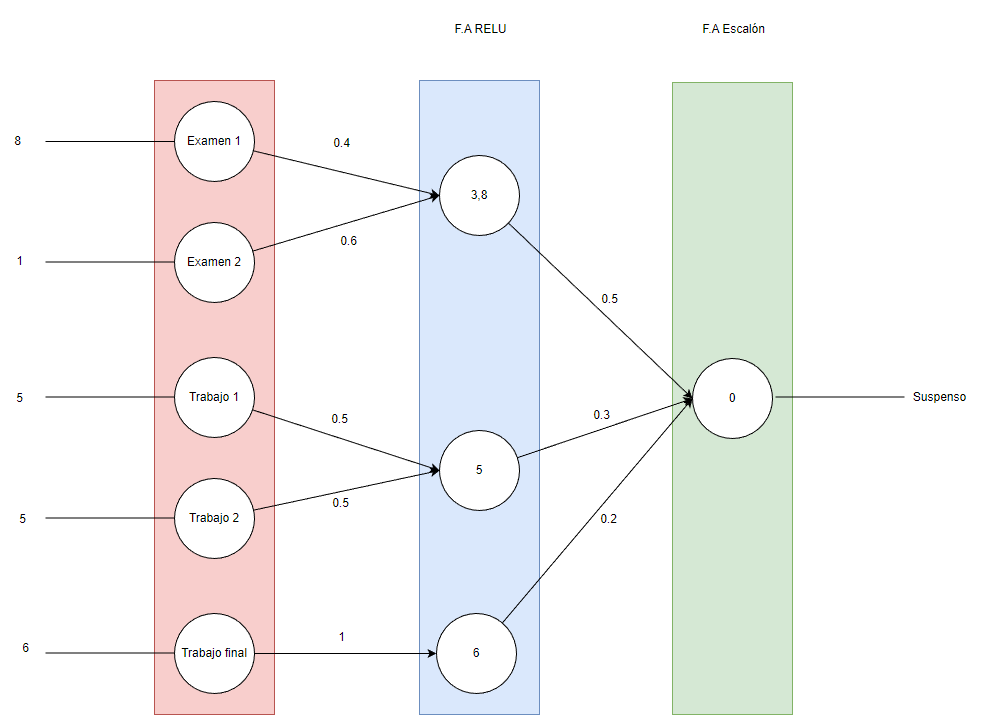
\includegraphics[width=0.9\textwidth]{img/Ejemplo Red Neuronal.png}
         \caption{Ejemplo de una red neuronal}
         \label{fig:ejemploRedNeuronal}
    \end{figure}
    
     Dentro de las redes neuronales, se encuentran las redes neuronales convolucionales (CNN), estas redes son las que poseen al menos una capa convolucional, consistiendo en la combinación de capas convolucionales, capas de agrupación y capas densas~\cite{definicion_CNN}.

     Una capa convolucional es un conjunto de neuronas artificiales que realizan varias series de operaciones convolucionales, actuando cada una sobre una submatriz de la matriz de entrada~\cite{definicionConvolucional_layer}.
     
     Una operación convolucional es aquella que a partir de una submatriz de la matriz de entrada (donde a veces es necesario realizar un filtrado para ponderar los datos) se calcula la suma de los valores de esta submatriz asignando el resultado a la matriz de salida~\cite{definicionConvolutional_Operation}.
     
     La capa de agrupación es una capa de una red neuronal que reduce el tamaño de la matriz de entrada, mediante operaciones como el máximo o la media de los valores de una submatriz~\cite{definicion_pooling}.

     La capa densa también llamada capa totalmente conectada, es una capa oculta, donde cada nodo está conectado a todos los nodos de la siguiente capa oculta~\cite{definicion_fully_connected_layer}.
     
    Una red neuronal residual es aquella que permite el salto de capas intermedias. Estas conexiones permiten que la red aprenda las características residuales, es decir, las diferencias entre las entradas y las salidas esperadas.  Para ello, se crea un bloque residual, que en lugar de transmitir la salida de una capa directamente a la siguiente, se introduce una conexión residual que suma la salida de una capa a la entrada de otra capa posterior como se puede ver en \ref{fig:residual-block}.

\begin{figure}[!ht]
         \centering
         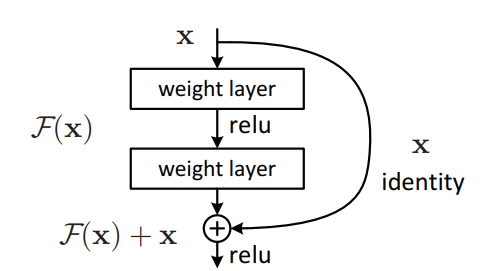
\includegraphics[width=0.6\textwidth]{img/residual-block.png}
         \caption{Bloque residual. Imagen extraída de~\cite{DBLP:journals/corr/HeZRS15}.}
         \label{fig:residual-block}
\end{figure}
\section{Preprocesado}
En el proyecto, se han realizado varios preprocesados, puesto que hay varias redes neuronales convolucionales.

\subsection{Red neuronal convolucional VGG16, para la calidad de la imagen}

En una red neuronal convolucional VGG16, el preprocesado necesario es que la imagen en vez de estar en formato RGB (Rojo, verde y azul), está en un formato BGR(Azul, verde y rojo), donde la diferencia entre estos formatos es el orden en el que se encuentran los colores, y en el preprocesado, también es necesario que los valores finales estén centralizados en 0. Además de este cambio, la imagen debe tener de 224 x 224 píxeles, redimensionando las imágenes que se introduzcan a la red.
\cite{tensorflowVGG16}
Para realizar este preprocesado en Python, se puede llamar a la función \textit{tf.keras.applications.vgg16.preprocess\_input}, para la aplicación de Android Studio, se ha implementado este preprocesamiento.
La estructura de la red convolucional VGG16, se puede observar en la figura \ref{fig:VGG-16-struct}, donde hay 13 capas convolucionales, y  4 de agrupación. 
\begin{figure}[!ht]
         \centering
         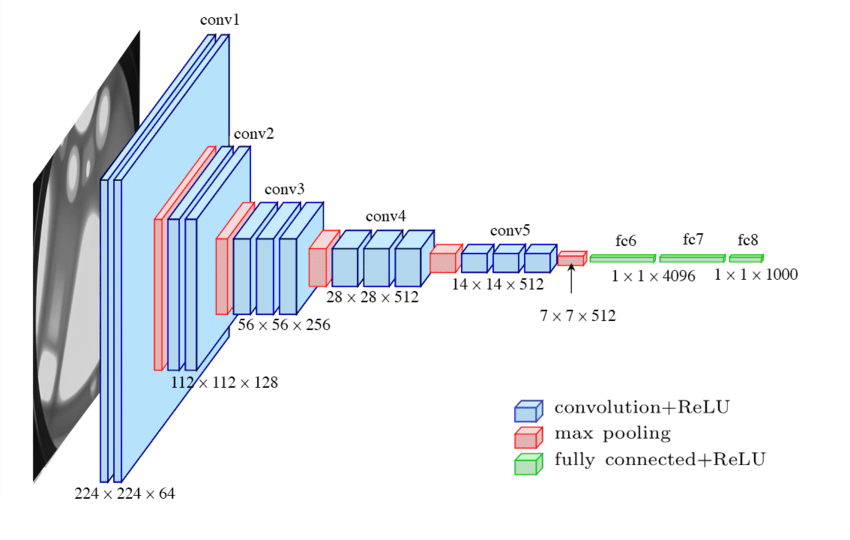
\includegraphics[width=0.9\textwidth]{img/VGG-16-network-architecture.png}
         \caption{Estructura básica de la red convolucional VGG16. Imagen extraída de~\cite{vgg16-structure}}
         \label{fig:VGG-16-struct}
\end{figure}


\subsection{Red neuronal convolucional ResNet50V2, para la detección de retinopatía}

La red ResNet50V2 es una red neuronal residual que, como se ha comentado anteriormente, permite saltarse capas, como se puede ver en la figura~\ref{fig:residual-block}.

En la red neuronal convolucional ResNet50V2, el procesamiento es distinto al de VGG16, la gama de color es RGB, también se tiene que normalizar los datos, pero en este caso, el intervalo es [-1,1]~\cite{tensorflowResNet50V2}.

Esta red neuronal ya estaba entrenada, por tanto, no se tuvo que hacer ningún preprocesado en Python; pero al implementar la red en Android Studio, al igual que en la red VGG16, se debía realizar el preprocesamiento a mano.

Donde la formula para cambiar este valor vendría dada por: 
\begin{center}
    $ColorPreprocesado = (ColorSinPreprocesar - 0)/ 255.0 * 2 - 1$
    \begin{itemize}
        \item Donde 0 representa el valor mínimo que puede tomar el color en concreto.
        \item Donde 255 representa el valor máximo que puede tomar el color en concreto.
        \item Y donde $ * 2 - 1 $ es la operación para normalizar el valor en formato [-1, 1]
    \end{itemize}
\end{center}

La estructura de la red convolucional ResNet50V2, se puede observar en la figura~\ref{fig:ResNet50v2-struct}, en esta red neuronal convolucional,  hay 50 capas repartidas entre 5 bloques. El primer bloque no es convolucional, pero los otros 4 sí que contienen capas convolucionales de tamaños variados, incluyendo convoluciones de 1x1, 3x3 y 1x1.
\begin{figure}[!ht]
         \centering
         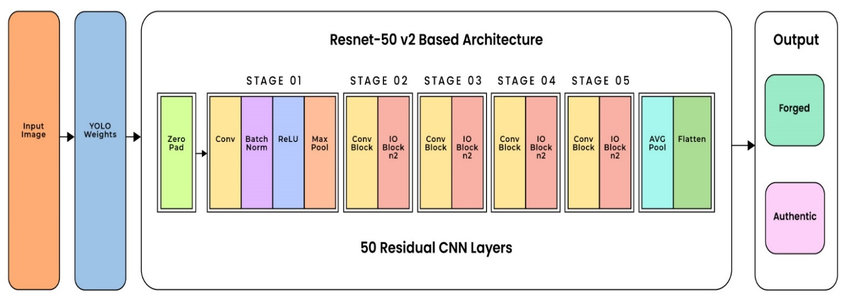
\includegraphics[width=0.9\textwidth]{img/ResNet50v2-architecture.jpg}
         \caption{Estructura básica de la red convolucional ResNet50v2. Imagen extraída de~\cite{ResNet50v2-architecture}}
         \label{fig:ResNet50v2-struct}
\end{figure}

\section{Transfer learning}

El aprendizaje transferido o ``Transfer learning'' es una técnica del \textit{Machine learning}, la cual consiste en reutilizar el conocimiento ya aprendido de un modelo, en otra actividad que tenga un objetivo similar. 

En el ámbito que nos concierne, se ha utilizado el modelo VGG-16 que ha sido entrenado con el dataset de ImageNet ``Large Scale Visual Recognition Challenge 2014 (ILSVRC2014) ''. El objetivo de este modelo es clasificar imágenes entre 1.000 categorías distintas, aprendiendo las características visuales de cada una. 

Para transferir el modelo, es necesario congelar las capas, para que no se entrenen. Con esto realizado, solo falta obtener el resultado, que puede ser binario o multiclase dependiendo del problema.

Además, se ha agregado una capa de agrupación para hacer uso de las capas densas. La primera capa densa consta de 64 neuronas con una función de activación RELU. Por otro lado, la segunda capa densa actúa como la capa de salida, y su propósito es evaluar la calidad de la imagen.

El código de creación del modelo sería el siguiente:

\lstset{
  language=Python,
  basicstyle=\small\ttfamily,
  keywordstyle=\color{blue},
  commentstyle=\color{green!60!black},
  stringstyle=\color{red},
  showstringspaces=false,
  breaklines=true,
  breakatwhitespace=true,
  tabsize=4,
  numbers=none,
  numberstyle=\tiny,
  frame=single,
  framexleftmargin=5mm,
  xleftmargin=5mm
}
\begin{lstlisting}
vgg16 = VGG16(include_top=False, weights='imagenet', input_shape=(224, 224, 3))
for layer in vgg16.layers:
    layer.trainable = False
model = Sequential()
model.add(vgg16)
model.add(tensorflow.keras.layers.Flatten())
model.add(tensorflow.keras.layers.Dense(64, activation='relu'))
model.add(tensorflow.keras.layers.Dense(num_classes, activation='sigmoid'))

\end{lstlisting}

\section{Formato de la red neuronal}

El formato de las redes neuronales convolucionales suele venir dado en formato ``.h5'' o keras, para facilitar la implementación en Android Studio, se ha tenido que transformar este archivo en formato TensorFlow Lite, el cual requiere menos recursos, permitiendo su integración en dispositivos móviles.

Para realizar esta conversión, se ha utilizado un fichero Python, el cual se ha buscado en la documentación de TensorFlow Lite, y posteriormente, guardar el fichero~\cite{tensorflowliteConverter}.

En el siguiente código, se puede observar el convertidor, donde file es el directorio donde se encontraría el archivo keras, nombre es el nombre de este fichero, y fileSalida es el directorio de salida.
\lstset{
  language=Python,
  basicstyle=\ttfamily,
  keywordstyle=\color{blue},
  commentstyle=\color{green!60!black},
  stringstyle=\color{red},
  showstringspaces=false,
  breaklines=true,
  breakatwhitespace=true,
  tabsize=4,
  numbers=none,
  numberstyle=\tiny,
  frame=single,
  framexleftmargin=5mm,
  xleftmargin=5mm
}
\begin{lstlisting}
model = tf.keras.models.load_model(file+nombre+'.h5')
converter = tf.lite.TFLiteConverter.from_keras_model(model)
tflite_model= converter.convert()
nombreSalida = "calidad.tflite"
with open(fileSalida+nombre+'.tflite', 'wb') as f:
    f.write(tflite_model)

\end{lstlisting}
\section{Desbalanceo de los datos}

Para la minería de datos, el problema de que los datos estén desbalanceados causa que los modelos entrenados suelan producir resultados indebidos.

Un ejemplo del desbalanceo de datos, podría ser un modelo que entrena los números diciendo si son primos o no. En este caso, si se calcula el modelo por porcentaje de aciertos, en caso de devolver siempre que el número introducido no es primo, esta medida tiende a ser del 100\%.
Por este motivo, se suelen usar otras métricas u otras formas de entrenar al modelo, para que se evite la disparidad de los datos.

La forma de solucionar este problema en este trabajo ha sido usando otras medidas como podrían ser precisión, recall y F1Score.
En la figura \ref{fig:matrizDeConfusion} se puede observar la matriz de confusión de positivos y negativos. A partir de la cual, se explicaran las medidas.
\begin{figure}[!ht]
         \centering
         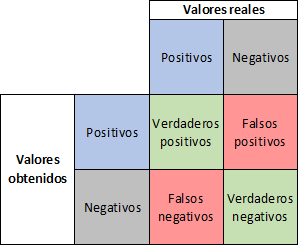
\includegraphics[width=0.6\textwidth]{img/Matriz de confusion.png}
          \caption{Matriz de confusión}
         \label{fig:matrizDeConfusion}
\end{figure}

La precisión es el numero de Verdaderos positivos entre la suma de verdaderos positivos y falsos positivos.
\begin{center}
    $Precision = \dfrac{Verdaderos Positivos} {Verdaderos Positivos + Falsos Positivos} $
\end{center}

Por otro lado, el recall, es el número de verdaderos positivos entre la suma de los verdaderos positivos y los falsos negativos.
\begin{center}
    $Recall = \dfrac{Verdaderos Positivos} {Verdaderos Positivos + Falsos Negativos} $
\end{center}

F1 Score es una medida obtenida de las dos anteriores, siendo la media armónica de estas.
\begin{center}
    $F_1 = 2 \dfrac{Precision * Recall} {Precision + Recall} $
\end{center}

En el caso concreto, una imagen puede ser APTA o NO\_APTA, encontrándose el desbalanceo de imágenes de 455 APTA y 103 NO\_APTA. De esta forma, se ha considerado en la matriz \ref{fig:matrizDeConfusion}, como ``Positivos'' a la clase NO\_APTA y como ``Negativos'' a la clase APTA.

La otra opción que no se ha utilizado, pero es importante destacarla, es el uso de oversampling o undersampling. Estas técnicas buscan igualar número de entidades en el conjunto de datos según la clase. 

Mientras oversampling, busca añadir datos a partir del conjunto de datos, duplicando o modificando los datos entre distintas instancias. Esta opción no se ha ni planteado, puesto que si se duplican las imágenes NO\_APTA, lo que va a producir es sobreajuste del modelo; y suponiendo que los datos nuevos fuesen modificaciones de combinaciones de imágenes  NO\_APTA, se estaría introduciendo ruido, puesto que crearía imágenes no reales.

El undersampling al contrario que el oversampling, elimina datos del grupo mayoritario, hasta que hay un número similar de instancias, las instancias eliminadas se pueden utilizar para validación o para test. Al implementar este método, se pueden eliminar inicialmente instancias que clasifican muy bien el modelo, haciendo que dependa el código de la inicialización del conjunto de entrenamiento y del conjunto de test.

\section{Guías de diseño Android}

Para realizar la aplicación se siguió la guía de diseño de Google Material3.

En los botones, se recomienda la forma circular en las esquinas, de forma que sea más visible para los ojos. En la figura \ref{fig:EsquinasRedondeadas} se puede ver la comparación entre las esquinas con pico y redondeadas, en esta explica que las formas con esquinas hacen que el enfoque esté fuera del rectángulo, mientras que en las redondeadas consigue que el enfoque esté dentro.
        \begin{figure}[!ht]
                 \centering
                 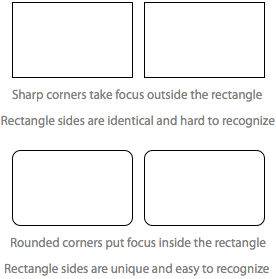
\includegraphics[width=0.45\textwidth]{img/rounded-corners.png}
                  \caption{Diferencias esquinas. Imagen obtenida de~\cite{rounded-corners-uxmovement}}
                 \label{fig:EsquinasRedondeadas}
        \end{figure}

Para los colores de la aplicación, como es una aplicación orientada en el bienestar y salud de las personas, estos colores tenían que ser claros con tonos verdes y azules, colores usados también en el diseño del logo de la aplicación, por otro lado, hay personas que prefieren un fondo oscuro a uno claro, por lo que se incluyo la opción de modo oscuro en la aplicación.

La gamma de color usada fue: en modo claro, gris claro para el fondo \#E0E0E0 y los botones azules claros \#90CAF9,  y para el modo oscuro, gris oscuro para el fondo \#353740 y los botones verdes claros.
Para el color del texto, varía entre blanco y negro según el fondo. Buscando en todo momento contraste  entre los objetos y el fondo de la aplicación.

Durante la ejecución de la aplicación, es preferible que los distintos objetos estén deshabilitados, a invisibles, de esta forma, el usuario entiende que si interactúa con la aplicación, ese objeto se habilitará. Como es el caso de la realización de la foto, que hasta que el usuario no haya seleccionado una imagen no puede pasar a la siguiente pantalla. Esto es contraproducente en algunos casos, puesto que los mensajes de error es mejor mostrarlos solo cuando el error ocurre; como es el caso de iniciar sesión incorrectamente o el caso de que la calidad de la imagen sea baja.
\capitulo{4}{Técnicas y herramientas}

\section{Metodologías}
\textbf{SCRUM}

    SCRUM es una metodología ágil basada en una estrategia continua e incremental, cuyo objetivo es proporcionar un producto funcional al final de cada periodo de trabajo planeado (\textit{sprint}), haciendo reuniones diarias y antes y después de cada \textit{sprint} otras reuniones donde se explican los problemas que se han tenido y como se va a planear el siguiente.

    El impedimento más notorio de esta metodología, es que hay un equipo de personas entre las que se encuentra el \textit{product owner}, el \textit{SCRUM master} y el equipo de desarrollo. Además el equipo se recomienda ser de entre 3 a 9 personas para un buen desarrollo, por tanto, en este trabajo ha sido complicado ir haciendo todas las acciones que se piden en la metodología SCRUM.

\textbf{GitFlow}

    GitFlow es un flujo de trabajo, en el cual se ramifica el proyecto en \textit{branches} donde cada una, contiene una parte del proyecto; de esta forma, se puede dejar una parte funcional sin modificar que seria la rama principal, y otras ramas, donde se van realizando los cambios, cuando en estas ramas, se termina la tarea que se esta realizando, haciendo un producto funcional, se realiza una operación de \textit{pull request} para combinar ambas ramas. Esta operación es aceptada o denegada por el equipo de desarrollo que no haya participado en la realización de esta rama.

    En mi proyecto, se han creado tres \textit{branches}, que son:
    \begin{itemize}
        \item \textit{main}: es la rama principal, donde se alberga la versión estable del proyecto.
        \item boceto: es una rama secundaria, donde se realizan los cambios que se están realizando en la aplicación móvil.
        \item latex: es la rama secundaria donde se realizan los cambios que se están realizando en el documento LaTeX.
    \end{itemize}
\textbf{Método del pato de goma}

    El método del pato de goma, o \textit{rubber duck debugging}, es un método informal para revisión de código.

    Este método es utilizado por muchos programadores y surgió porque normalmente los programadores han tenido experiencias donde han tenido que explicar el problema a otra persona que no entiende sobre programación, y mientras se esta explicando el código, encontrar posibles soluciones. 
    
    Por tanto, este método, consiste en vez de explicar el código a otra persona, en explicárselo a un pato de goma.

\section{Herramientas}

    \subsection{Repositorio}
        Entre las opciones para realizar el repositorio, se pensó en GitLab y en GitHub, tomando esta última por conocimiento de uso de esta.

        GitHub es una plataforma web de alojamiento de repositorios que utiliza Git como sistema de control de versiones.

        Por tanto, como GitHub utiliza Git de forma nativa, no fue necesario la elección de un sistema de control de versiones porque ya estaba incluido.
    \subsection{Gestión del proyecto}
        Entre las opciones para gestionar el proyecto, se pensó en poder realizarlo con GitHub Projects, con Jira, con ZenHub y Trello; tomando la opción de ZenHub, por ya estar familiarizado con la herramienta.

        ZenHub es una herramienta de gestión de proyectos que se integra con GitHub. Proporciona una tabla Kanban, donde se ponen las actividades a realizar durante el \textit{sprint}. Permite poner una prioridad a las tareas, siguiendo una estimación de poker, y además, ofrece la posibilidad de ver gráficos \textit{burndown} donde se representa las actividades que faltan por hacer en el \textit{sprint}, también ofrece otros gráficos como \textit{cumulative flow} y \textit{velocity tracking}.

    \subsection{Guía de diseño}
        Para la realización de la aplicación, es necesario una guía de diseño que facilite al usuario la interacción con la aplicación. Por ello, se utilizo la ultima guía ofrecida por Google, llamada Material 3.

        Material 3 es la ultima versión del sistema de diseño del \textit{open source} de Google.
        En el documento, viene información de recomendación de componentes ante el mismo problema.

    \subsection{Herramienta de iconos}
        Para la adición de iconos en la aplicación, es necesario que las imágenes y o iconos sean \textit{open source} para ello, se estuvieron mirando páginas que ofrecían estos iconos, entre las páginas, al final se seleccionaron pixabay para la obtención de imágenes, puesto que ofrece licencia de uso para proyectos comerciales y no comerciales.

        Por otro lado, para los iconos se utilizó Google Fonts y la galería que ofrece Android por defecto, se utilizo Google Fonts, porque en la guía de desarrollo se recomendaba y a su vez, es de código abierto y gratuito.

        Para el logotipo de la aplicación, se ha utilizado DALL-E, una inteligencia artificial que convierte texto a imágenes, tras varios intentos, se logró conseguir un logotipo bastante bueno, y con ello, se hicieron unos retoques con el uso del programa de edición de imágenes GIMP, para la eliminación de ruido y para proporcionarle una gamma de colores; como resultado se obtuvo el icono actual.

    \subsection{Entorno de desarrollo integrado (IDE)}
        Para el desarrollo de la aplicación móvil, se pensó en Eclipse, Android Studio y Unity.

        Al final, se descarto Eclipse por no ofrecer una experiencia de desarrollo especifica para aplicaciones Android. Y también se descarto Unity, aunque Unity si que esta especializado en aplicaciones móviles, por otro lado, se especializa en el desarrollo de videojuegos y en aplicaciones con realidad virtual.
        Por lo tanto, se selecciono Android Studio, es el IDE oficial de Android y está desarrollado por Google, basado en IntelliJ IDEA. Ofrece un emulador donde se compila la aplicación y poder comprobar el correcto funcionamiento de esta.
        Además, para la compilación hace uso de Gradle, separando el código de la aplicación, de la compilación.

        El lenguaje utilizado ha sido Java, aunque Android Studio ofrece la opción de Kotlin, con Java no hacia falta aprender un nuevo lenguaje, puesto que se ha cursado durante la carrera.

    \subsection{LaTeX}
        Para la realización del documento, se pensó utilizar MiKTeX, TeX Live u Overleaf.
    
        Al final, se escogió Overleaf, puesto que las otras 2 herramientas eran locales, y Overleaf ofrece acceso desde la nube, además tiene integración con proyectos GitHub, facilitando la exportación al repositorio.


    \subsection{Comunicación}
        Para la comunicación con los tutores, se uso tanto email, como tutorías presenciales, de esta forma, las cuestiones y los avances realizados se hacen por email, y en caso de mostrar el funcionamiento de la aplicación o alguna duda más importante, se realiza presencialmente para un mejor entendimiento.

\section{Patrones de diseño}
    \subsection{Modelo-Vista-Presentador}
        Es una derivación del patrón modelo-vista-controlador, la diferencia es que se cambia el controlador por un presentador, el cual sirve como intermediario entre el modelo y la interfaz.
        \begin{itemize}
            \item El modelo, define los datos que se utilizan en la interfaz.
            \item El presentador, funciona como intermediario, recuperando los datos del modelo, y cambiando la vista de la interfaz.
            \item La vista, es la interfaz de usuario.
        \end{itemize}
        Puesto que Android Studio, ya proporciona separaciones para hacer uso de un modelo-vista-presentador, su implementación ha sido sencilla, donde las \textit{activities} son las diferentes interfaces, los archivos java del directorio "com.example.retinopatia" son los presentadores de las vistas, y en el directorio DataBase se encuentra el modelo de datos.


\capitulo{5}{Aspectos relevantes del desarrollo del proyecto}

Este apartado pretende recoger los aspectos más interesantes del desarrollo del proyecto, comentados por los autores del mismo.
Debe incluir desde la exposición del ciclo de vida utilizado, hasta los detalles de mayor relevancia de las fases de análisis, diseño e implementación.
Se busca que no sea una mera operación de copiar y pegar diagramas y extractos del código fuente, sino que realmente se justifiquen los caminos de solución que se han tomado, especialmente aquellos que no sean triviales.
Puede ser el lugar más adecuado para documentar los aspectos más interesantes del diseño y de la implementación, con un mayor hincapié en aspectos tales como el tipo de arquitectura elegido, los índices de las tablas de la base de datos, normalización y desnormalización, distribución en ficheros3, reglas de negocio dentro de las bases de datos (EDVHV GH GDWRV DFWLYDV), aspectos de desarrollo relacionados con el WWW...
Este apartado, debe convertirse en el resumen de la experiencia práctica del proyecto, y por sí mismo justifica que la memoria se convierta en un documento útil, fuente de referencia para los autores, los tutores y futuros alumnos.

\capitulo{6}{Trabajos relacionados}

\section{Proyectos}
    \subsection{Ret-iN CaM}
    \href{https://apps.apple.com/us/app/ret-in-cam/id1509765945}{Ret-iN CaM} es la aplicación que se ha tomado de referencia para hacer el proyecto. Es una aplicación iOS que posteriormente saco una versión para Android. Es una aplicación que permite realizar imágenes y vídeos de la retina con una gran resolución, proporcionando los informes del paciente, los cuales se pueden exportar para ser compartidos con otros especialistas.
    A su vez, tiene una interfaz simple e intuitiva, lo que facilita a los usuarios interactuar fácilmente con ella. Principal motivo por el que se ha escogido esta aplicación.

    \subsection{D-EYE}
    \href{https://www.d-eyecare.com/}{D-EYE} es un proyecto que permite la toma de imágenes y vídeos de alta calidad; permite a los médicos ver el nervio óptico sin necesidad de dilatar las pupilas; permite a los médicos ver si el paciente tiene trastornos neurológicos relacionados con el ojo.

\newpage

\section{Comparativa del proyecto}
\begin{table}[htbp]
\centering
\begin{tabular}{lccc}
\toprule
Características & RetinAI & Ret-iN CaM & D-EYE \\
\midrule
 
Aplicación Android & X & X & \\
Aplicación iOS & & X & X \\
Creación de usuarios  & & & X \\
Cambio de modo oscuro y claro & X & & \\
Permite iniciar sesión como invitado & X &   &   \\
Permite guardar la sesión  &  & X & X \\
Permite elegir el paciente & X & X & X \\
Ver historial del paciente & X & X & X \\
Crear nuevos informes & X & X & X \\
Permite diferenciar entre ojos  & X & X & X \\
Permite hacer imágenes & X & X & X \\
Permite hacer vídeos & & X & X \\
Escoger imágenes desde la galería & X &  & \\
Red neuronal para los resultados & X &  &  \\
Versión gratuita & X & X & X \\

\bottomrule
\end{tabular}
\caption{Comparativa de las características de los proyectos.}
\label{comparativa-proyectos}
\end{table}

De esta forma, se puede ver las ventajas que ofrece el proyecto.
\begin{itemize}
    \item Actualmente, hay más móviles con sistema operativo Android que con iOS, por tanto, se ha realizado la aplicación en un sistema Android por este motivo.
    \item No se permite la creación de usuarios, puesto que como la aplicación esta destinada a médicos de la sanidad publica, la entidad encargada les proporcionará las cuentas para la aplicación.
    \item La aplicación tiene la opción de cambiar entre modo oscuro y modo claro, de esta forma, permite al usuario adaptarla a su preferencia.
    \item Al iniciar sesión como usuario, los médicos podrán tener un diagnostico rápido de un paciente, sin que se almacene el informe en la base de datos.
    \item A la hora de seleccionar pacientes, se ha considerado la protección de datos de los pacientes y para que el médico seleccione a uno, tendrá que poner el DNI.
    \item Como es posible que se analice una foto tomada desde otro dispositivo. Se ha considerado esta idea mostrando en el explorador de archivos las imágenes.
    \item Ofrece una red neuronal ya entrenada, la cual determina el grado de retinopatía diabética que tiene el paciente. Característica en la que se basa la aplicación.
    
\end{itemize}

\capitulo{7}{Conclusiones y Líneas de trabajo futuras}

En este apartado, se desarrolla las conclusiones obtenidas del proyecto realizado y los futuros usos o cambios a añadir al proyecto.

\section{Conclusiones}

A continuación se muestra una lista de las conclusiones que se pueden obtener de este trabajo:

\begin{itemize}
    \item Se han cumplido todos los objetivos planteados al inicio del documento, descartando el objetivo de agilizar el sistema sanitario, puesto que no se ha distribuido la aplicación, y en el caso de haberlo hecho, y que el sistema sanitario español quiera esta aplicación, la agilización no se podría percibir hasta pasado un tiempo.

    \item El uso de Android Studio ha aportado facilidades en el desarrollo de la aplicación, donde la documentación ha sido un factor clave. Por otro lado, el intento de que la aplicación pueda ejecutarse en el máximo número de dispositivos, ha conseguido que la aplicación no este optimizada, con herramientas especificas de ultimas versiones.

    \item Muchos de los conceptos vistos en el proyecto, se han visto durante la carrera, profundizando conceptos como las redes neuronales, la interacción con la aplicación, bases de datos,...

    \item Antes de la realización de este proyecto, no se miraba la documentación de las herramientas utilizadas, y en la mayoría de casos, ayudan a resolver las dudas que se tienen. 

    \item La utilización de una metodología ágil en este proyecto no se ha notado, puesto que no hay cliente y no se cambian los requisitos a lo largo del tiempo, ocurre lo mismo con el SCRUM master, como no hay un equipo como tal, siendo todos los actores la misma persona, todas las reuniones se han omitido y además, la estimación de las tareas es complicada, porque no se tiene un conocimiento previo de las tareas, y porque es un proyecto individual, es decir, con más personas se podría estimar por media. Por tanto, no creo que sea recomendable esta metodología para este tipo de proyectos individuales.

\end{itemize}

Finalmente, se ha conseguido una aplicación funcional que permite a los médicos, o al personal identificado, obtener resultados sobre la imagen capturada. Además, se ha añadido el modelo que detecta si una imagen tiene una calidad correcta, para que de esta forma, no se generen expedientes con una calidad mala, donde el resultado puede no ser el real. 

En este caso, el usuario no tiene que ser experto en aplicaciones Android, ni en redes neuronales; donde se deja elegir al médico lar red neuronal, se debería explicar en que ocasiones es mejor cada una.

\section{Líneas de trabajo futuras}

El origen de la aplicación surge de la utilización de esta en el sistema sanitario publico, por lo que se propone utilizar esta aplicación como base sobre la que trabajar. 

\subsection{Base de datos}

En primer lugar, será necesario cambiar la base de datos esto es así, porque SQLite permite crear bases de datos locales, y en caso de que se quiera acceder a un expediente creado desde otro dispositivo móvil, no existiría. Por este motivo, se debería conectar la aplicación a una base de datos online.

\subsection{Redes neuronales convolucionales}

Otro posible cambio, son las redes neuronales, en caso de obtener nuevas redes neuronales más precisas, o que consuman menos recursos, se pueden o añadir, cambiando la vista de la interfaz, añadiendo una nueva opción para el modelo; o también se podría cambiar una de las actuales, borrando el modelo anterior, y añadiendo el nuevo.

Además, en un futuro, se aumentará el conjunto de datos, permitiendo a las redes neuronales 

\subsection{Añadir versiones Android}

Actualmente, la aplicación se puede ejecutar desde dispositivos Android con una API mayor a 21, se podría aumentar el número de dispositivos disponibles, y por otro lado, es posible que en estos dispositivos, al tener distinta resolución que los dispositivos actuales, sea necesario ajustar el contexto xml dinámicamente.

\subsection{Aumentar el número de sistemas operativos}

El proyecto ha sido creado para Android, aumentar el número de dispositivos, para que los usuarios no se vean obligados a utilizar un teléfono Android. 

Siendo la opción más recomendable añadir una versión para iOS.

\subsection{Distribución}

Actualmente, no se ha implementado una opción para distribuir la aplicación y que el usuario pueda descargarla.

Se recomienda el uso de Play Store, puesto que es la distribuidora oficial de Android y la más usada por los usuarios de Android.

\subsection{Uso de la aplicación por el paciente}

La aplicación ha sido desarrollada con el objetivo de ser usada por los médicos, en un futuro, se podría dar soporte también a los pacientes, donde podrían ver los informes, o incluso en caso de tener el hardware hacer la propia toma proporcionándole una guía de como hacerlo correctamente.

\subsection{Idiomas}

Como el proyecto surgió con la idea de ser utilizado en el servicio sanitario publico español, el único idioma implementado ha sido el castellano; en un futuro se podrían llegar a añadir las lenguas cooficiales como catalán, gallego y euskera.

En caso de querer internacionalizar la aplicación, añadir en cualquier caso el inglés, y posteriormente, los idiomas oficiales de los países donde se vaya a usar la aplicación.

\subsection{Actualizaciones}

Como la aplicación trata sobre la salud de las personas, los cuales pertenecen al grupo de categorías especiales de datos personales según el Reglamento General de Protección de Datos; es importante que todas las actualizaciones comprueben que no se puede filtrar los datos; y en caso de que pueda ser así, sacar una nueva actualización rápidamente.

\subsection{Tests unitarios}

Como durante el proyecto se valoraba más la interacción del usuario con la aplicación, se realizaron test manuales. De esta forma, se podrían implementar tests automáticos para comprobar el correcto funcionamiento.


\bibliographystyle{plainnat}
\bibliography{bibliografia}


\end{document}
